\documentclass{school-22.211-notes}
\date{February  8, 2012}

\begin{document}
\maketitle

\lecture{Introduction}
\topic{Course Coverage}
\begin{itemize}
  \item Calculation of neutron spectra;
  \item Resonance absorption and spatial self-shielding models;
  \item Continuous energy transport, reduction to multi-group diffusion group;
  \item Determination of few-group diffusion constants;
  \item Elementary reactor transient analysis.
\end{itemize}

\begin{table}[ht]
  \centering
  \begin{tabular}{|p{1in}|p{2in}|p{0.65in}|p{0.6in}|p{1.5in}|} \hline
    Topics & Break down  & This notes & Reuss & Other Text \\ \hline
    %
    \multicolumn{1}{|c|}{\multirow{2}{*}{Calculating Spectra}} & Slowing down \& thermalization in infinite medium   & Ch.~\ref{slowing-down-thermalization} & Ch.7, 9  & Duderstadt p.316-332, Hebert 4.2.3 \\ 
    & Resonance Models & Ch.~\ref{resonance-model-chap} & Ch.2.7, Ch.8 & Duderstadt p.333-347 \\ \hline
    %
    \multirow{3}{*}{Diffusion Equations} & Continuous energy derivation & Ch.~\ref{intro-to-diffusion-theory} & Ch.5, 6 & \\ 
    & One group: analytical & Ch.~\ref{1g-1}, Ch.~\ref{1g-criticality}, \ref{1g-source} & Ch.10  &  \\ 
    & Multi group: derivation, numerical solutions & Ch.~\ref{multi-group-diffusion},\ref{2g-finite-difference}, \ref{matrix-representation-of-1d-slab} & Ch.10  &  Stacy 3.10. \\ \hline
    %
   \multirow{5}{*}{Dynamics \& Kinetics} & Fission product, depletion & Ch.~\ref{fission-product-poisoning}, \ref{fuel-depletion} & Ch.11, 12 &  \\
    & PKEs, with and without feedback & Ch.~\ref{PKE-without-feedback}, \ref{PKE-with-feedback}  & Ch.4, 13 & \\
    & Nodal Methods  & Ch.~\ref{nodal-methods}  &  & Smith's paper \\
    & Homogenization, Dehomogenization & Ch.~\ref{homogenization}, \ref{de-homogenization}  &  &Smith, Palmtag, Rempse, Jiang \\
    & Adjoint, perturbation & Ch.~\ref{adjoint-fluxes} & Ch.16 & \\ \hline 
  \end{tabular}
  \caption{Topics Covered in This Class}
\end{table}



\clearpage
\topic{Sample Exercises}
\uline{Example 1: Estimate the Mean Free Path of a Fission Neutron in an LWR} 
\begin{figure}[ht]
  \centering
  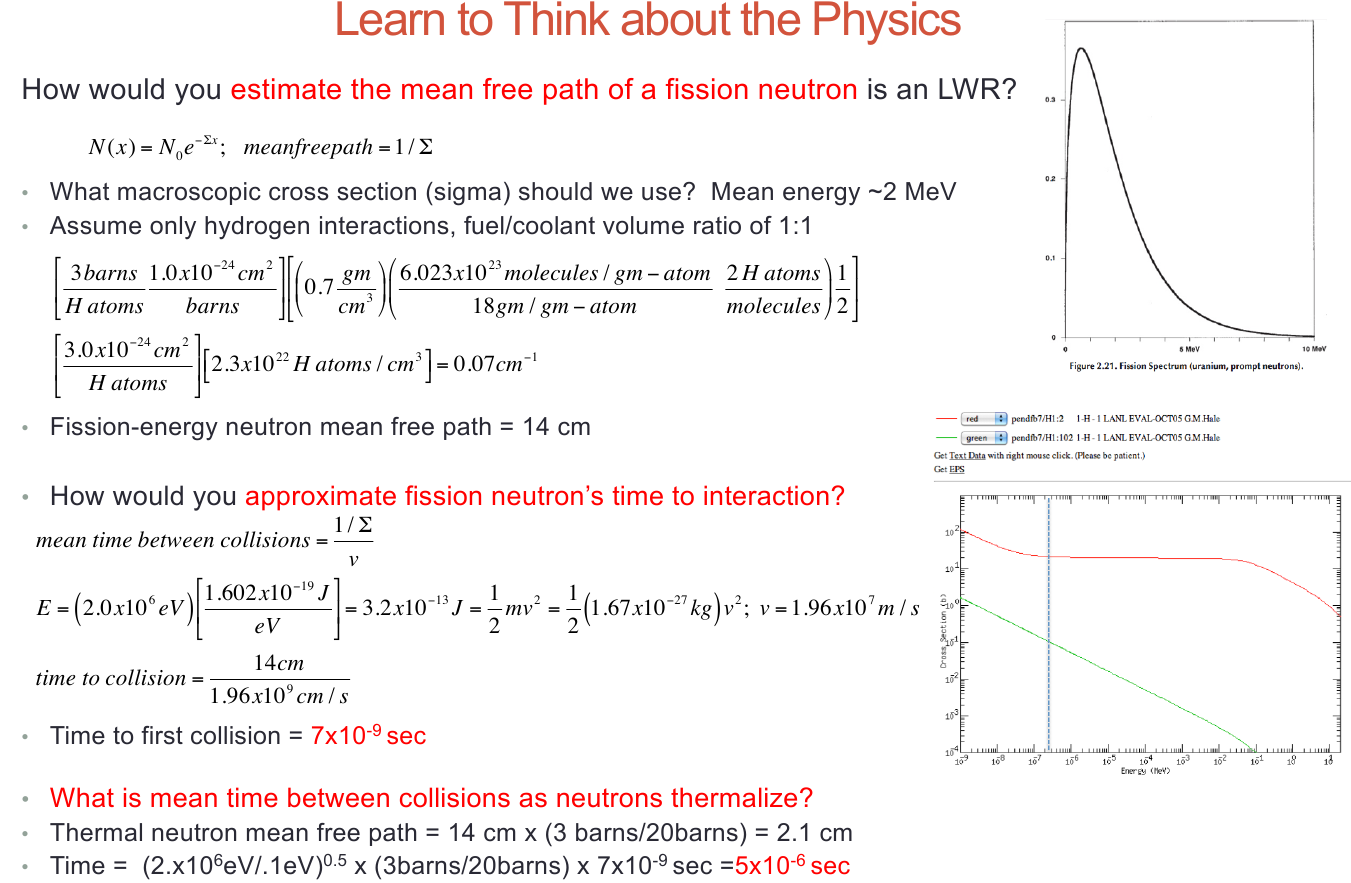
\includegraphics[width=5.5in]{images/intro/lec1-example1.png}
\end{figure}

\clearpage
\uline{Example 2: Estimate Prompt Neutron Lifetime}
\begin{figure}[ht]
  \centering
  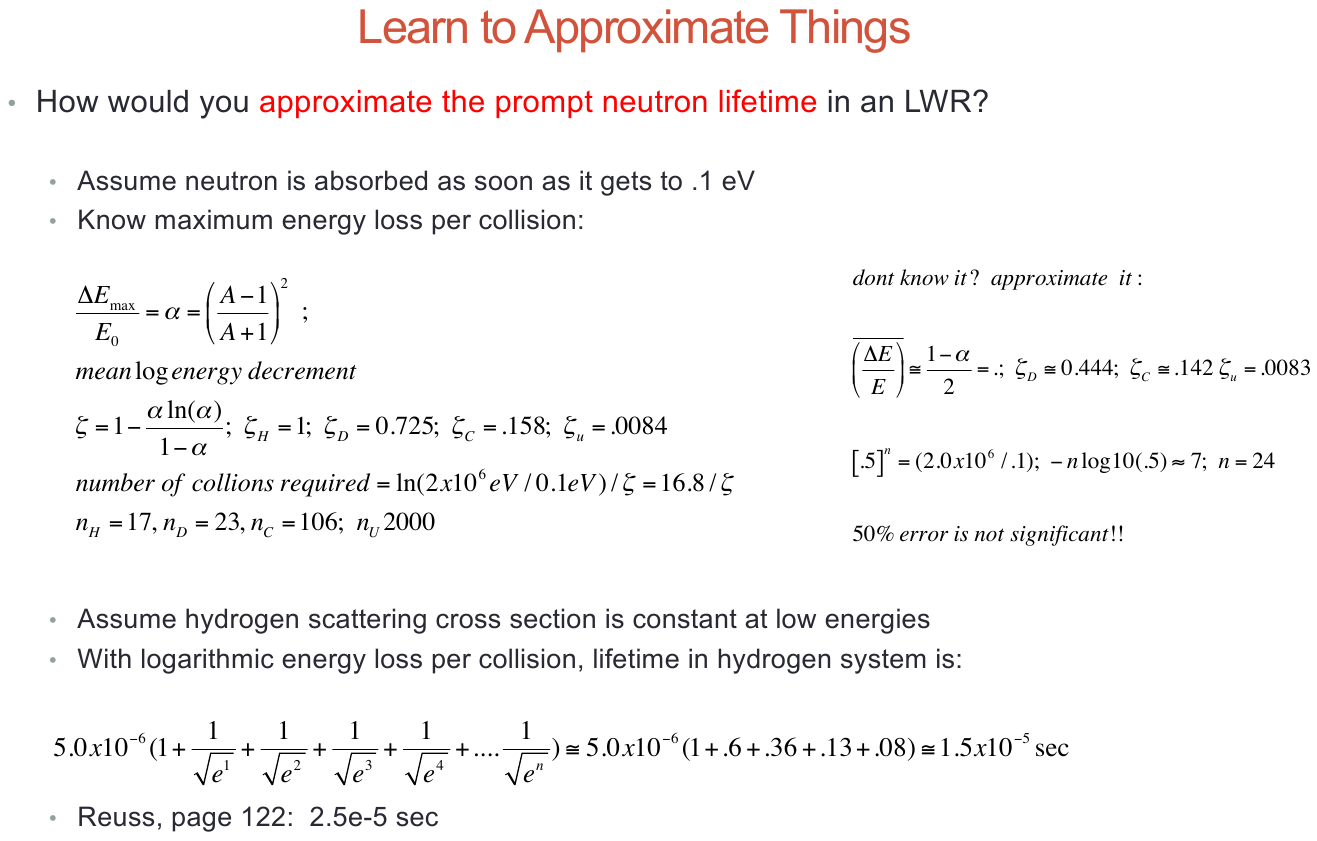
\includegraphics[width=4.5in]{images/intro/lec1-example2.png}
\end{figure}

\uline{Example 3: Estimate Fast \& Thermal Fluxes in an LWR}
\begin{figure}[ht]
  \centering
  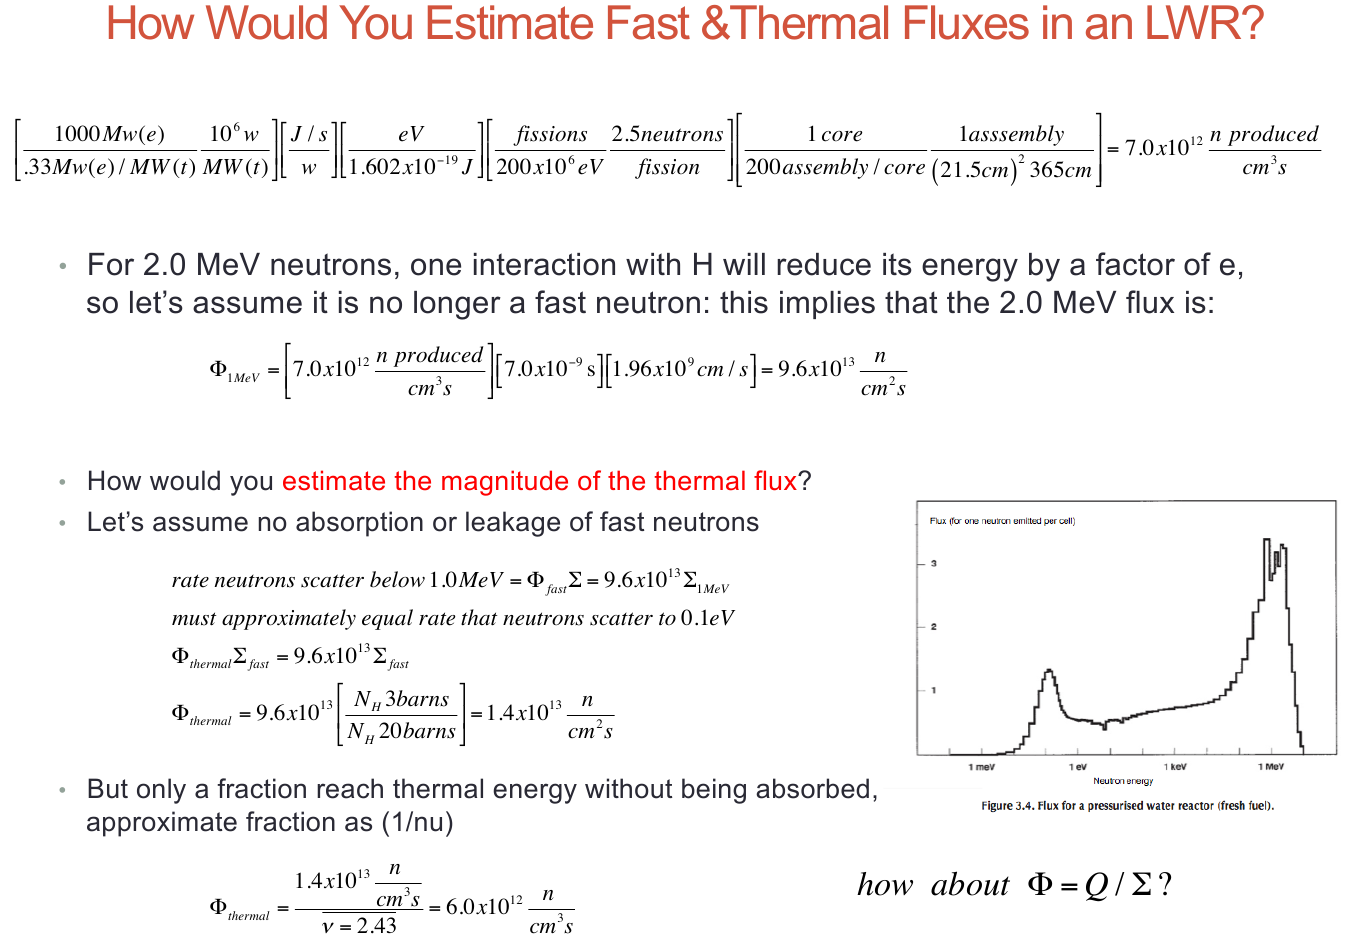
\includegraphics[width=4.5in]{images/intro/lec1-example3.png}
\end{figure}

\clearpage
%%%%%%%%%%%%%%%%%%%%%%% Begin of Ch 1 %%%%%%%%%%%%%%%%%%%%%%%%%% 
\topic{Summary: Reuss Ch 1 History}
\begin{enumerate}
\item Carnot efficiency $r_{\mathrm{max}} = 1 - \frac{T_{\mathrm{cold}}}{T_{\mathrm{hot}}}$. 
\item Moderator choice: low neutron capture, light nuclei to slow down neutrons, sufficienty dense (1.5). 
\end{enumerate}
%%%%%%%%%%%%%%%%%%%%%%% End of Ch 1 %%%%%%%%%%%%%%%%%%%%%%%%%%%% 

%%%%%%%%%%%%%%%%%%%%%%% Begin of Ch 2 %%%%%%%%%%%%%%%%%%%%%%%%%% 
\topic{Summary: Reuss Ch 2 Intro to Nuclear Physics}
This chapter goes over some basic nuclear physics concepts which we just covered in 101 so I am going to skip most of them and note on concepts that I did not remember.
\begin{enumerate}
\item Stable and unstable nuclei (2.1.4): all elements beyond bismuth (Z=83) are radioactive; there are no stable isotopes found in nature for Z = 43 and Z = 61. 
\item Mass defect $\Delta m = Z m_p + N m_N - m_A$. Nuclear binding energy: $W = \Delta m c^2$. 
\item Liquid drop model: $W = a_v A - a_s A^{2/3} - a_a \frac{(A/2 - Z)^2}{A} - a_c \frac{Z^2}{A^{1/3}} + \delta a_p A^{-1/2}.$ Even-even: $\delta = 1$; odd-odd, $\delta = -1$; else, $\delta = 0$. 
\item Spin: even-even nuclei have zero spin, and can be approximately as spherical; even-odd nuclei have spin of $n+1/2$; odd-odd nuclei have integer number of spin. 
\item The width of the excited states is related to their lifetime $\tau$ by Heisenberg uncertainty $\Gamma \tau \approx \hbar$, which decreases we increase the excitation energies, until a continuum zone where the levels overlap. 
\item Positive mass defect (initial mass $>$ final mass): exoenergetic/exothermic reaction; otherwise, endothermic reaction. 
\item Law of radioactive decay: $N(t) = N(0) e^{-\lambda t}, T = \frac{\ln 2}{\lambda}$. Meanlife $=\frac{1}{\lambda}$ is the average amount of time after which an unstable nucleus observed at a given instant will disintegrate.  
\item Examples of radioactive decay (2.4.4).
\item THe interaction probability element for a path $\dx$ is $\Sigma \dx$. Mean free path $\lambda$ is the average distance at which the first collision occurs:
\eqn{ \lambda = \expect{x} = \int_0^{\infty} x p(x) \dx = \int_0^{\infty} x \exp{-\Sigma x} \Sigma \dx = \frac{1}{\Sigma} }
\item Main reactions, see Table~\ref{main-reactions} (2.6.3).
  \begin{table}
    \centering
    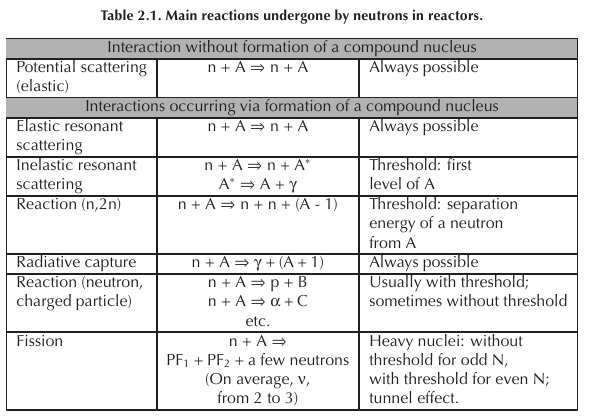
\includegraphics[width=5in]{images/intro/main-reactions.png}
    \caption{Main Reactions Undergone By Neutrons} \label{main-reactions}
  \end{table}
\item Cross sections: $\sigma_a = \sigma_f + \sigma_c, \sigma_t = \sigma_a + \sigma_s$. 
  \begin{itemize}
  \item Absorption cross sections (radiative capture, fission, $(n,p), (n,\alpha)$) often follow 1/v behavior in the thermal range (less than 1 eV). 
  \item Scattering cross sections tend to be constant corresponding to the potential scattering (the geometric value of the image of the target and the projectile), plus possible resonances especially for intermediate and heavy nuclides. $\sigma_{\mathrm{pot}}$ is about a few barns, with the only exception being H with the largest scattering cross section of 20 barns. 
  \end{itemize}
\item Fission barrier (2.9.2). Parity effect (2.9.3): the binding energy is much greater when the initial target has an odd number of neutrons than an even number. Application: \ce{^{235}U}'s 6.5 MeV binding energy overweights its fission barrier of 6.1 MeV, hence making fissioning easy; on the contrast, \ce{^{238}U}'s binding energy 4.8 MeV is smaller than its 6.6 MeV fission barrier. 
\item Tunnelling (2.9.4): even if the excitation energy of the compound nucleus is smaller than the barrier, fission can still occurs through tunneling. 
\item Prompt neutron fission spectrum (2.10.1): Maxwell spectrum, Cranberg spectrum, etc. Energy released in fission (2.10.3). 
\end{enumerate}
%%%%%%%%%%%%%%%%%%%%%%% End of Ch 2 %%%%%%%%%%%%%%%%%%%%%%%%%%%% 

\clearpage
%%%%%%%%%%%%%%%%%%%%%%% Begin of Ch 3 %%%%%%%%%%%%%%%%%%%%%%%%%% 
\topic{Summary: Reuss Ch 3 Intro to Neutron Physics}
\begin{enumerate}
\item Flux $\Phi = n v$, the population of neutrons travelling through the matter (3.1.1). 
\item Current $\vec{J}(\vec{\Omega}) = \vec{v} n(\vec{\Omega}) = v \vec{\Omega} n(\Omega) = \vec{\Omega} \Phi(\Omega).$
\item Mean chord: the average distance separating the point of exit from the point of entry of a neutron crossing the area under consideration, $l = \frac{4V}{S}$. The opacity of the area $\omega = \frac{4V\Sigma}{S}$ (3.1.5). 
\item The Boltzmann equation (3.1.6): 
\eqn{ \Phi(\vec{r}) = \int \frac{e^{-\tau}}{4 \pi R^2} \left[ \nu \Sigma_f(\vec{r}') \Phi(\vec{r}')  + \Sigma_s(\vec{r}') \Phi(\vec{r}') \right] \derivative^3 r'} 
Operators associated with the Boltzmann equation (3.2.3).
\item Neutron spectra (3.3.1):
  \begin{itemize}
  \item Fast reactors: the spectrum is degraded with respect to the fission spectrum. Reason: slowing down by inelastic scattering off heavy nuclei and elastic scattering off sodium.
  \item Thermal reactors: 
    \begin{enumerate}
      \item a high energy hump. Reason: fission spectrum, degraded due to scattering; 
      \item slight decrease in the epithermal region. Reason: resonant capture losses, esp. U238; 
      \item  a low energy hump. Reason: Maxwell distribution of the thermal agitation but a little harder because the temperature equilibrium has not been perfectly achieved. 
    \end{enumerate}
  \end{itemize}
\item Four factor formula (3.3.2). 
\end{enumerate}
%%%%%%%%%%%%%%%%%%%%%%% End of Ch 3 %%%%%%%%%%%%%%%%%%%%%%%%%%%% 




\end{document}
